\begin{savequote}[75mm]
Nothing in Biology Makes Sense Except in the Light of Evolution
\qauthor{Theodosius Dobzhansky}
\end{savequote}

\chapter{Introduction}
\label{introduction}
\begin{flushleft}
\setlength{\parindent}{7ex}
\section{Disclosure}
Parts of this introduction, especially the section on Wnt signaling, have been adapted from own publications, including \textit{Wnt signaling in cancer} \cite{Zhan2017}

\section{The Colon}
\subsection{Colon Function and Value as Model Organ}


evolutionary fundamental value
representative model for complex organ
well understood stem cell biology enabled modeling in vitro 
devastating diseases emerge from colon

\subsection{The Colon Stem Cell Niche}
In order to understand the underlying principles of colorectal cancer development, or any cancer in general, it is advisable to turn to the stem cell biology governing the tissue's anatomy and function. The colon stem cell niche, or crypt, is the source of all epithelial cells lining the colon. Similar to the small intestine, Lgr5+ instestinal stemcells are located at the bottom of the crypt and continuously renew the epithelium by proliferating and pushing out new cells towards the colon's lumen.

This architecture serves multiple purposes, including protection of stem cells and the control of cell fate decisions across the epithelium. Multiple developmental pathways, especially Wnt signaling, Notch, BMP and ERK MAPK signaling, govern cell identity in the intestinal niche \cite{Gehart2019}. The concentration of signaling cues for most of these pathways are organized in gradients along the crypt-lumen axis. For example, the concentration of stem cell property maintaining Wnt and EGF ligands, secreted by mesenchymal crypt cells and REG4+ deep secretory cells, decreases as cells are pushed outside of the crypt  \cite{Sasaki2016}. In contrast, the effect of cell differentiating BMP ligands increases as the effect basal mesenchmymal cell derived BMP inhibitors, such as Noggin, is reduced. In summary, as a cell is pushed outside the crypt by a continuous stream of fresh proliferating cells, developmental signaling cues vanish and subsequent gene expression changes lead to differentiation. Similarly, if cells were to move back into the crypt, the ambient signaling would lead to a reprogramming towards an intestinal stem cell fate. 

Given the spacial confinement of proliferate signals, the crypt architecture leads to a protection against malignant transformation, too. At the bottom of the crypt, a neutral competition of proliferating intestinal stem cells leads to the rapid removal of cells that show reductions in their proliferation rate relative to wildtype stem cells, which is often the case in malignant neoplasms. Given this neutral competition and the dependence on external signaling, every dysfunctional or transformed cell is likely removed from the niche and differentiates unless it acquires a set of molecular alterations that render it independent from niche signals. As mentioned above, the key signaling pathways that maintain stem cell properties in the crypt are canonical Wnt signaling and Notch signaling, while BMP signaling inhibits stemness and EGF dependent ERK MAPK signaling triggers cell proliferation. Given their exerted evolutionary pressure on malignant cells, it comes at no suprise that the majority of early driver mutations found in colorectal cancer, such as loss of APC (Wnt signaling), activation of \textbeta-catenin (Wnt signaling), activation of KRAS (ERK MAPK), BRAF (ERK MAPK) and loss of SMAD4 (TGFb/BMP signaling) are found in these exact signaling pathways. Of these mutations, especially mutations of APC and KRAS are frequently observed early in colorectal cancer development and are highly correlated with eachother (50\% of APC mutant tumors harbor mutations of KRAS), leading to both induced proliferative capacity and growth. In summary, the architecture of the colon stem cell niche and the signaling pathways required to regulate stemness and cell proliferation influence the evolutionary landscape of colorectal cancer development and thus account for the majority of early drive mutations, especially loss of APC and activation of KRAS, in this disease.

\subsection{Signaling Pathways controlling the Colon Stem Cell Niche}
\subsubsection{Canonical Wnt Signaling}
In 1973, the wingless gene was discovered in a screen for visual phenotypes, affecting patterning processes in Drosophila melanogaster, the fruit fly \cite{Sharma1973WinglessMelanogaster.}. Subsequently, further genetic screens identified components of the Wnt family as key regulators during embryonic development and later, cancer initiation as well as stem cell maintanance  \cite{Nusslein-Volhard1980MutationsDrosophila}. \par 

In canonical Wnt signaling, absence of Wnt ligands leads to phosphorylation of \textbeta-catenin by the destruction complex, which contains the scaffold protein Axin, the large protein APC (Adenomatous polyposis coli) and the kinases GSK3\textbeta as well as casein kinase (CK1\textalpha) (reviewed in Zhan, Rindtorff et al.\cite{Zhan2017}). 
In this state, \textbeta-catenin is phosphorylated by GSK3\textbeta, ubiquitinated by \textbeta-TrCP and subsequently targeted for proteasomal degradation. 
In the absence of nuclear \textbeta-catenin, the trasncritpional repressive complex containing TCF/LEF and transducing-like enhancer protein (TLE/Groucho) recruits Histone deacetylases to repress target genes. \par 

The canonical pathway is activated upon binding of secreted Wnt ligands (for example, Wnt1 and Wnt 3a) to Fzd receptors and LRP co-receptors. 
Subsequently, LRP receptors are  phosphorylated by CK1\textalpha and GSK3\textbeta, which then recruits Dishevelled (Dvl) proteins to the plasma membrane where they polymerize and are activated \cite{Metcalfe2011}. Next, the Dvl polymers inactivate the destruction complex by sequestration in multivesicular bodies. This results in stabilization and accumulation of \textbeta-catenin which then translocates into the nucleus. There, \textbeta-catenin forms an active complex with LEF (lymphoid enhancer factor) and TCF (T-cell factor) proteins by displacing TLE/Groucho complexes which leads to the recruitment of histone modifying co-activators such as CBP/p300, BRG1, BCL9 and Pygo \cite{Lien2014WntSignaling}. \par 

Next to Wnt ligands, members of the R-spondin ligand family are positive effectors of Wnt signaling \cite{Kazanskaya2004, Glinka2011, Hao2012}. R-spondins bind to leucine-rich repeat containing G-protein-coupled receptors (Lgr) 4-6 \cite{Koo2012a}. In the absence of R-spondin, the two E3 ubiquitin ligases Znrf3 and Rnf43 target the Frizzled (Fzd) receptor for lysosomal degradation \cite{DeLau2011}. The interaction of ubiquitin ligases and receptrs is dependent on Dishevelled (Dsh).\cite{Jiang2015}. In the presence of external R-Spondins, binding of ligands to Lgr4-6 inhibits the activity of Znrf3/ Rnf43 and leads to the accumulation of Fzd receptors on the cell surface \cite{Hao2012, Koo2012a}. Being transcriptional targets of Wnt signaling, Znrf3 and Rnf43 function as negative feedback regulators in Lgr5- positive cells \cite{DeLau2012}. \par 


\subsubsection{ERK MAPK Signaling}
The extracellular-signal-regulated (ERK) mitogen-activated protein kinase family (MAPK) is one of three major MAPK families, together with the JNK (c-jun N-terminal kinase or stress-activated protein kinases) and MAPK14 group of protein kinases. These signaling cascades play a major role in (I) integrating external proliferative signals, (II) reacting to stress or ambient cytokines and (III) protecting cells from apoptosis, respectively \cite{Oncol2005}. 


\subsubsection{IGF and mTOR Signaling}

\subsubsection{TGF beta Signaling}

\subsubsection{TP53 Signaling}

\subsection{Colon Organoid models}
Intestinal organoids are three-dimensional cell culture models from primary adult tissue. Organoids develop from Lgr5+ adult stem cells and were first isolated from the small intestine of mice \cite{Sato2011}. Subsequently, following the initial methodology, further organoid models across tissue-types and species have been developed. These include organoids from intact and cancerous human large intestine \cite{Sato2011}, pancreas \cite{Sachs2017}, mammary epithelium \cite{Zhang2016EstablishingCells, Sachs2017AHeterogeneity}and the hepatobiliary system \cite{Huch2013NIHAccess, Broutier2016CultureManipulation.}.
Culturing these cells requires the addition of specific tissue-dependent growth factors and the embedding of cell in 3D hydrogels \cite{Merker2016GastrointestinalOut}. In the case of colon organoids, the necessary growth factors are inspired by signaling cues available in the intestinal stem cell niche: Wnt and R-spondin ligands secreted by PDGFR+ myofibroblasts activate and maintain canonical Wnt signaling; EGF ligands stimulate ERK MAPK signaling and Noggin ligands inhibit the differentiating effects of the BMP signaling cascade \cite{Sato2013}. When combined with inhibitors of TGF\textbeta and p38 mediated signaling, these growth factors can stimulate the formation and continous proliferatation of organoids ex-vivo. 

Not only because of their high isolation efficancy of up to 80\%, organoids are an increasingly popular model as they mimic their respective tissue of origin, including colorectal cancer (Pauli et al. 2017). Due to a high isolation efficiency and preserved tumor biology, patient derived colorectal cancer organoids have been used as personalized cancer models for precision oncology \cite{VanDeWetering2015, Vlachogiannis2018}. Moreover, organoids from healthy tissue can be cultured in-vitro as well and are amenable to genetic editing (Matano et al. 2015 Drost et al. (2015)). Therefore, these models also enable studying tumor development at a single mutation resolution.

\section{Colorectal Cancer}
\subsection{Colorectal Cancer Epidemiology}
Colorectal cancer is the third most common cancer worldwide and is associated with a Western lifestyle. Similar to other solid tumors, colorectal adenocarcinoma progression is classified into four stages by the UICC (Union for International Cancer Control). These range from a \textit{carcinoma-in-situ}, a malignant patch of cells that has not yet breached the basal lamina of the intestinal mucosa (stage 0), to metastatic disease (stage 4).\par


\begin{figure}[h]
\centering
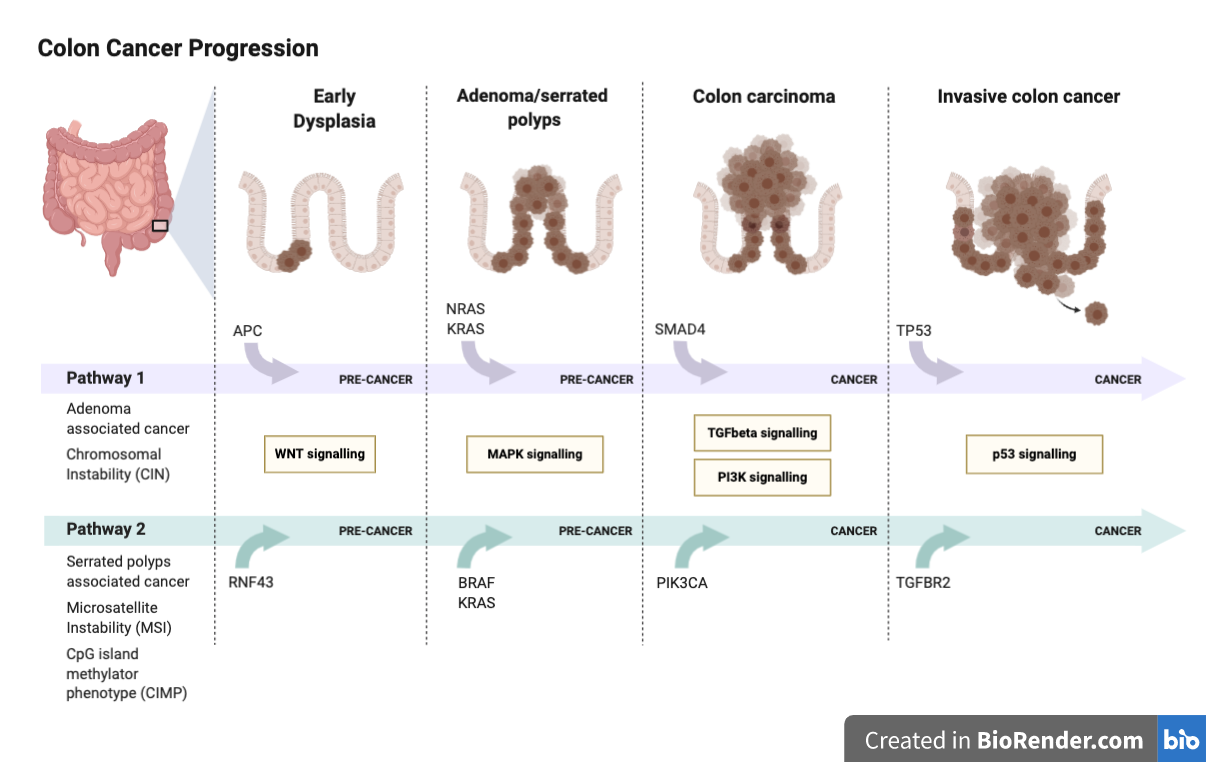
\includegraphics[scale=.35]{figures/colon_cancer_progression.png}
\caption{Colon Cancer Progression}
\label{colon_cancer_progression}
\end{figure}

\subsection{Colorectal Cancer Emergence and Evolution}
According to the adenoma-carcinoma sequence model, the majority of all colorectal adenocarcinomas arise from previously formed adenomas, benign neoplasms of the intestinal epithelium \cite{Cho1992}. Thus, today, one of the most effective medical interventions to reduce death from colorectal cancer is the preventative removal of visible adenomas during lower endoscopy, such as colonoscopy \cite{Nishihara2013Long-TermEndoscopy}.\par

On a molecular level, colorectal adenocarcinoma can be organized into tumors arising through (I) a chromosomal instability or (II) a DNA-mismatch repair deficiency associated route \cite{Markowitz2009} (Figure \ref{colon_cancer_progression}). These two forms of tumor development have been associated with characteristic clinical, pathological and molecular findings. For example, tumors of the DNA-mismatch repair phenotype are more frequently located in the right colon, have a higher proportion of microsatellite instability, frequent BRAF mutations and a higher immune-cell infiltration \cite{Markowitz2009}. In contrast, tumors of the common chromosomal instability (CIN) phenotype are mostly microsatellite stable and have frequent APC and KRAS mutations. \par 

The cascade of genetic events leading to the more frequent chromosomal instability associated form of colorectal cancer cause hyperactivation of a range of signaling pathways. Briefly, this cascade, known as the Vogelstein sequence \cite{Cho1992}, starts with the loss of the tumor suppressor APC in the intestinal epithelium. Loss of APC, which leads to adenoma formation, is followed by the activation of KRAS, PIK3CA, loss of SMAD4 and TP53. Other forms of the disease, especially microsatellite-instable forms of colorectal cancer also harbor mutations of APC but show strong prevalence of BRAF mutations instead of KRAS mutations \cite{Guinney2015TheCancer.}. \par 

Prior studies trying to further define colorectal cancer beyond these two developmental routes have proposed a set of different molecular subtypes \cite{Menter}. In an attempt to unify these models, four consensus molecular subtypes (CMS) have been proposed \cite{Guinney2015TheCancer.}. Briefly, these subtypes organize colorectal cancer into classes defined by (I) a high fraction of microsatellite instable tumors, (II) APC mutations, (III) KRAS mutations and (IV) stromal infiltration, respectively. However, recent evidence has questioned the interpretability of these subtypes in multiple ways. First, the existence of non-malignant cells within the analyzed samples does not allow a direct interpretation of cancer-exclusive molecular processes which might govern treatment response and prognosis \cite{Dunne}. Second, the sampled intra-tumor region and its cellular composition influence the subtype classification result \cite{Dunne2016ChallengingCancer.}. Third, validating studies of the consensus molecular subtype have shown that a large fraction of cancer samples can not be confidently assigned to a single subtype and, more importantly, that subtypes, instead of being well separated, are rather on a high-dimensional continuum. This continuum can be defined by (I) markers of inflammation and T-cell activity and (II) markers of CDK-regulated DNA replication, leading to four quadrants in a continuous space \cite{Ma}. For example, microsatellite instable tumors, which are most frequently found in the first CMS subgroup, were associated with a strong T-cell activity signature and a low CDK-regulated DNA replication signature. Along these lines, immune-cell infiltration has been established as an independent prognostic factor of overall survival and recurrence risk of colorectal cancer and is exploited in immunotherapy, which is especially active in MSI-high tumors \cite{galon, pages}. In contrast, CDK-dependent signaling has recently been recognized as a potential driver of immune-escape in multiple solid cancers \cite{Chaikovsky1}. \par 

In summary, the molecular landscape of colorectal cancer is organized by two distinct forms of tumor development, chromosomal instability and microsatellite instability, that are linked to characteristic genetic changes resulting in a continuum of gene expression states which present themselves with varying degrees of cell proliferation and inflammation. \par

\subsection{Signaling Pathways controlling Colorectal Cancer}
\subsubsection{Wnt signaling in colorectal cancer}
The role of Wnt signaling during colorectal cancer development is well established \cite{Polakis2007}. While activating mutations of \textbeta-catenin do exist, loss of APC is the most frequent driver of Wnt signaling in colorectal cancer and can be found in about 80\% of colorectal cancer patients \cite{Fearon1989}. In line with its role as a tumor suppressor, truncating of APC using the CRISPR/Cas9 technology, leads to colorectal cancer development, which can be modeled ex vivo in human intestinal organoids \cite{Matano2015, Drost2015SequentialCells}. Furthermore, by using a mouse model allowing the reversible knockdown of Apc via shRNA, it was demonstrated that adenomas could regress to normal tissue once APC function is restored, underlining the importance of continuous Wnt signaling for tumor maintenance \cite{Dow2015}. \par
Although loss of APC in general is a driving event of colorectal cancer development and persistence, not every mutation of the APC gene leads to a similar phenotype. Studies of human colorectal cancer samples and tumors from mouse models revealed that different mutations of APC result in distinct levels of canonical Wnt pathway activity and, in addition, are associated with characteristic tumor locations within the large intestine \cite{Christie2013, Buchert2010}. \par

Besides APC, mutations in R-spondin and RNF43, regulators of Wnt receptor abundance at the cell surface level, 
were implicated as drivers of Wnt-dependent tumor growth. Deleterious RNF43 mutations have been described in ~20\% of colorectal cancer cases and are mutually exclusive to APC mutations. Also, amplified R-spondin3 fusion proteins have been described in 10\% of CRC cases. While APC and \textbeta-catenin are generally considered independent of Wnt ligand availability, RNF43 mutant cancers are strongly dependent on Wnt secretion, rendering them highly susceptible to Wnt secretion targeted therapy.

\subsubsection{ERK MAPK Signaling in Colorectal cancer}


In colorectal cancer, the ERK MAPK signaling cascade and its members Ras/Raf/MEK and ERK are key regulators of cell proliferation in malignant cells. The Ras kinase members are mutated in about 36\% of colorectal cancers \cite{Oncol2005}. According to the Vogelstein model of colorectal cancer initiation \cite{Fearon1989}, activating mutations of KRAS takes place early during cancer development, more specifically, after loss of APC.
Next to KRAS, BRAF mutations can also be found in around 10\% of colorectal cancers \cite{Oncol2005}. Of note, mutations of KRAS and BRAF occur mostly in a mutually exclusive pattern with BRAF mutations being enriched in Microsatellite instable colorectal cancers \cite{Oncol2005, Sahin2013}. 

\subsubsection{IGF and mTOR Signaling in Colorectal Cancer}

\subsubsection{TGF beta Signaling in Colorectal cancer}

\subsubsection{TP53 Signaling in Colorectal cancer}

\subsection{Colorectal Cancer Organoid models}

\section{Colorectal Cancer Therapy}
The treatment of colorectal adenocarcinoma depends on disease stage. While surgical removal of the tumor is at the center of the treatment strategy, neoadjuvant and adjuvant chemotherapy are part of the recommended therapy from UICC stage 2 and 4 on, respectively. Today, for metastatic colorectal cancer the first line treatment includes combination chemotherapy (FOLFOX or FOLFIRI) paired with Cetuximab (anti-EGFR) for KRAS wildtype disease, combination chemotherapy with Bevacizumab (anti-VEGFR) for KRAS mutant disease or triple chemotherapy (FOLFOXIRI) in combination with Bevacizumab for BRAF mutant disease \cite{Cutsem}. Following lines of therapy include different combinations of the aforementioned agents with the exception of Regorafenib and Triflouridin/Tipiracil as preferred third line agents for non-KRAS wildtype disease \cite{Cutsem}. Consequentially, the only genetic tests currently recommended during therapy are the determination of KRAS and BRAF status \cite{Cutsem}. Other genetic tests or targeted inhibitors have so far not found their way into clinical practice.\par

Both the important role of adenocarcinoma development and the limitations of personalized therapy in advanced stages of the disease motivated the research presented in this dissertation.

\section{Cancer Drug Discovery}
\subsection{Rational and Functional Drug Discovery}
\subsection{Image-based Profiling}
A challenge for organoid research is the need for information-rich drug-testing methods. In the past, automated microscopy of 2D-cells has been used to measure the biological activity of compounds (Breinig et al. 2015). Prompted by this, we build a platform for high-throughput drug activity profiling in organoids. The platform uses confocal microscopy to collect fluorescent images of treated organoids in 3D. We devel- oped SCOPE, a software package, to process these images and measure organoid phenotypes. We used this platform to test compounds on both patient derived organoids and genetically engineered organoid models.

\section{Multi-View Representation Learning in Biology}
PCA
CCA
MOFA
Theis lab papers
Schoelkopf causal representation learning and Fischer causal genetic interaction


\section{Aims of Thesis}
\subsection{Image-based profiling of colon organoid models}

Patient derived organoids (PDOs) are physiological 3D tumor models that can be efficiently derived from cancer and normal tissues.1–3 Organoid isolation from human primary tumors and metastases1,4 has enabled the establishment of living biobanks.2,3,5–7 Notably, patient derived organoids have been shown to represent their origin’s molecular features and morphology,2–4,8 enabling functional experiments such as drug testing ex vivo.3,5,9–14 
Image-based profiling is a high-throughput microscopy-based methodology to systematically measure phenotypes of in vitro models. By learning a lower dimensional representation of biological images, biological states can be described, quantified and deciphered. When scaled and combined with chemical or genetic perturbations, this becomes a powerful approach to gain systematic insights into biological processes, making it a popular method in drug discovery and functional genomics research.15–17. Image-based assays have for instance been used to screen large libraries of small molecules to identify potential drug candidates, to analyze a drugs mode of action, or to classify drug-gene interactions by cell-morphology.18–21 Recently, image-based profiling of monogenic disease models has been particularly relevant for drug discovery. Here, primary cells from diseased tissue are profiled, perturbed and candidate drugs reversing the phenotype from a diseased to a healthy cell morphology are prioritized for drug development or used as diagnostics.22,23
Previously, high-throughput image-based profiling experiments have mostly been performed in a limited number of adherent cell lines and not been available to a growing number of disease models that require more sophisticated culture conditions, such as models from diverse cancers, rare genotypes or personalized disease models. Performing image-based profiling experiments of patient derived cancer organoids, a prime example for a complex 3D polygenic disease model, are, however, a technical and biological challenge. While image-based drug testing in organoids have been performed, the morphological heterogeneity of patient-derived cancer organoids between and within patient donors as well as their diverging behavior upon molecular perturbations are not yet systematically understood.24–26
Here we report on a large-scale image based phenotyping study of patient derived cancer organoids. We generated patient derived organoids from colorectal cancer patients and treated 11 organoid models with more than 500 experimental and clinically used compounds at different concentrations. We systematically mapped the morphological heterogeneity of patient derived organoids and their response to compound perturbations from more  than  3,700,000  confocal microscopy images. We identified a heterogeneous landscape of organoid phenotypes mainly driven by differences in organoid size, viability and cystic vs. solid organoid architecture. Using multi-omics factor analysis, we identified biological programs underlying these phenotypes and compounds that modulate them. For example, we linked cystic organoid architecture with a LGR5+ enriched, Wnt signaling dependent organoid state that could be induced via MEK inhibition and organoid size to an IGF-1R driven organoid state that was relatively insensitive to EGFR inhibition and could be induced via mTOR inhibition. A better understanding of organoid phenotypes and the ability to use multi-omics data to annotate organoid states and their plasticity have the potential to further accelerate image-based drug discovery for complex multigenic diseases.


\subsection{patient derived organoids identifies compound-induced phenotypes}
\subsection{Multi-omics profiling of intestinal organoids identifies an epistatic relationship of Apc loss and Kras activation during colorectal cancer development}
\end{flushleft}

% First, we isolated and characterized patient derived colorectal cancer organoids. Next, we performed high- throughput drug profiling of these organoids. Here, we observed a variety of recurring treatment-induced phenotypes. These were linked to specific cellular processes. Of note, the treatment response of organoids in-vitro matched the response of donating patients.

% Second, we isolated colon organoids from healthy mouse tissue. By using gene-editing, we generated models of colon adenoma - a precursor lesion of colorectal cancer. These models carried different combinations of mutations in the Apc and Kras gene. Both are frequent and co-occurring mutations in colorectal cancer (Schell et al. 2016). To better understand the mechanisms of tumor development, we performed a multi- omics characterization in these adenoma models. Moreover, we profiled genotype specific drug effects. Here we found a reorganization of organoid phenotype after loss of Apc, which masks the effects of an isolated Kras mutation. Loss of Apc leads to genotype specific drug-induced phenotypes and vulnerabilities. Oncogenic Kras buffers a subset of these vulnerabilities, offering a new perspective on the relationship of Apc and Kras during tumor development.